\subsection*{Data Collection}

A Struck Integrated Systems (SIS) 3302 DAQ module was used to collect data. This module has 16-bit ADCs and an internal 100 MHz clock which was used for all of the measurements. Preamplifier output signals were fed directly to the DAQ module without additional processing. These output signals were digitized and used to perform this analysis. Additionally, the on-board shaping amplifier was used to retrieve event energies (in ADC units).

The trigger threshold value was set so that gamma-ray pulses with energies as low as approximately 50 keV could be collected without excessive noise and without exceeding the voltage range of the DAQ. Data was collected attempting to have negligible pile-up effects. The event rate was chosen to be approximately 800 Hz (triggers) for a system with a 100 MHz clock (10 ns sampling time) and a preamplifier pulse decay time of roughly 50 $\mu$s.

Before further processing each pulse was baseline corrected. This was done by subtracting the average value of the first 15 samples from all of the samples in that pulse.

\subsection*{Energy Calibration}

Before taking spectral data, each channel must be calibrated. The 661.7 keV line from ${}^{137}$Cs and the 59.5 keV line from ${}^{241}$Am were used to perform a linear energy calibration.

Four calibration data sets were taken. First an ${}^{241}$Am source was placed near the outward face of detector 1. Next, the source was moved to the outward source of the detector 2. This was repeated with a ${}^{137}$Cs source. This was done to ensure that all channels would have spectral data for both sources.

Two spectra were plotted for each channel, one using both ${}^{241}$Am data sets combined, and the other using both ${}^{137}$Cs data sets combined. A region of interest around each photopeak was selected by visual inspection of the relevant spectrum. These regions were each fit with a Gaussian function and a linear function (to account for background) using the built in models in LmFit \cite{LMFIT}. A linear energy calibration was used.

Channels which had fewer than 50 total counts around the ${}^{137}$Cs peak or showed other strange behavior (visually observed) in spectra were not calibrated, and were not used in any of the analysis shown. This included 28 of the 152 channels. Most of these channels correspond to strips near the edge of the detectors which have been disconnected due to high leakage currents. However, some are recoverable. With higher statistics or The channel the abnormally high FWHM value in figure \ref{fwhm} had very few events in the cesium photopeak region and a very flat distribution, leading to poor, inaccurate fitting. Channels which are not plotted were not calibrated.

The energy resolution of each channel is determined from the FWHM of the cesium peak. This is shown in figure \ref{fwhm}. Each individual channel had a relatively low number of counts in the photopeak. The error bars shown correspond to fitting errors. Low statistics in the peaks limited this procedure (there were roughly 60 counts for a single channel). The average energy resolution was found to be 2.39 keV., with a standard deviation of 0.39 keV. The channels with high FWHM values tend to be those with a small number of counts in the peak. The variation between channels would likely decrease with better statistics. Ideally, all strips would have the same energy resolution. Realistically, however, we expect that some strips, in particular those on the outer edges of the detector, to have degraded energy resolution. The DC face of detector 1 contains channels 0 through 37. Here we see a u-shaped trend in the energy resolution, potentially demonstrating the effects of higher leakage current near the edges. The DC face of detector two contains channels 38 through 75. Here we also see a slight u-shaped curve, though the trend is not definite. The AC face of detector 1 spans channels 76 through 113 and the AC face of detector 2 spans channels 114 to 151.

\begin{figure}
\begin{centering}
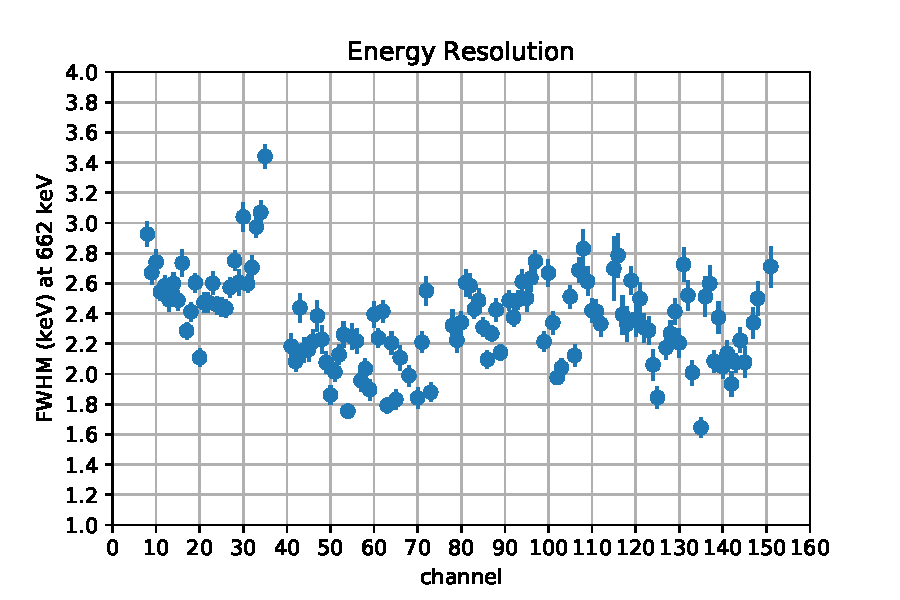
\includegraphics[width=0.7\textwidth]{./figures/energy_res.pdf}
\caption{The energy resolution for each channel of two double-sided strip detectors. Channels with a 0 FWHM are those which were not calibrated due to low statistics, high leakage currents, or other issues. The error bars shown correspond to fitting errors.}
\label{fwhm}
\end{centering}
\end{figure}

\subsection*{Timing}

For this and all following sections and analysis, the events used were for a ${}^{137}$Cs  source, positioned several decimeters away from the DC face of detector 1. ${}^{137}$Cs was used to ensure events throughout the potential range of detector depth. Additionally, these signals have greater SNR which makes it easier to properly trigger on and correlate signals.

A distribution of trigger times over all events and both detectors was plotted. For a Poisson process, the distribution of arrival times is exponential, peaked at zero and falling more steeply with increasing rate (the decay constant of the exponential function is $\lambda = 1/mean rate)$. 

The distribution for experimental triggers does not follow this trend exactly. There are more events near 0 and more events at 1 than at zero. t is found that most events occur within 20 nanoseconds of each other ($\approx$ 82 $\%$, as seen in figure \ref{timehist}. This is probably due to several effects. For each event which causes a trigger on a strip, it is very likely to see triggers on other strips. For each event, ideally we would see at least two strips trigger, at least one on each side of the detector. Due to charge sharing and image charges on neighboring strips, more than just these two strips can register an event. Additionally, triggers due to noise and random coincidences will also increase the rate of event triggers. Lastly, there is some uncertainty in the timestamps used to calculate the time between events. There is likely some variation in the trigger time recorded by the SIS modules, which will depend on the on-board fast trapezoidal filter (used for triggering) parameters and event topology. The effect of this was not evaluated in this work.

\begin{figure}
\begin{centering}
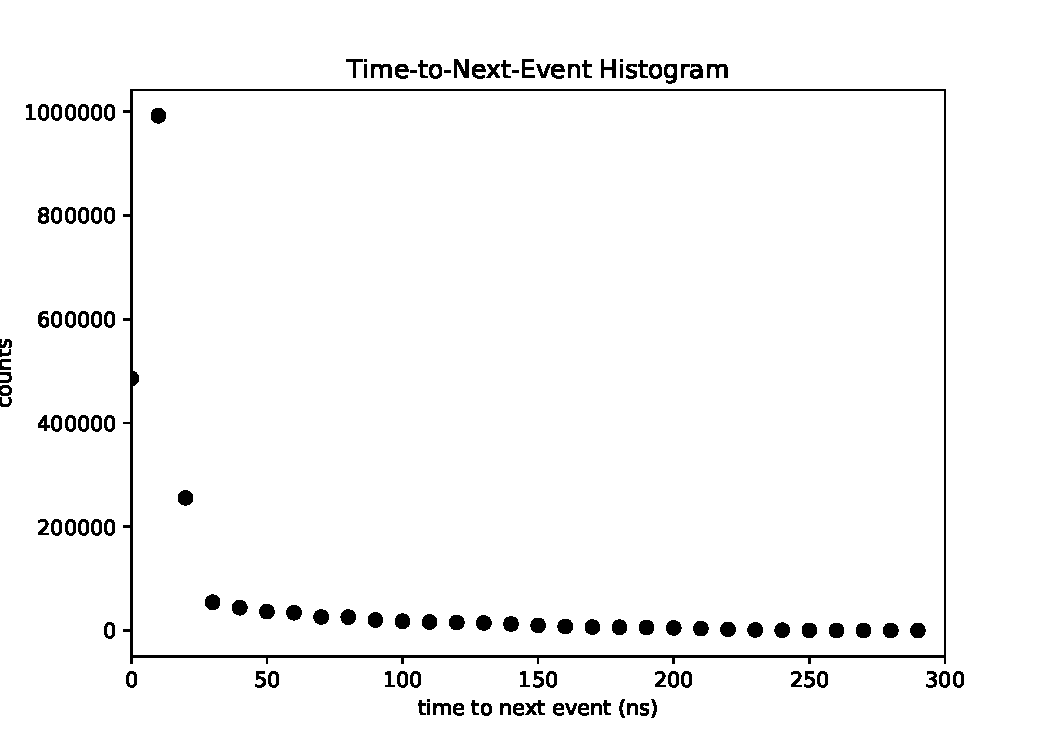
\includegraphics[width=0.7\textwidth]{./figures/time-to-next-event.pdf}
\caption{The time-to-next event histogram}
\label{timehist}
\end{centering}
\end{figure}

To select single-site events, events which have triggers within 70 ns of each other on opposite faces of a detector crystal were selected (see next subsection for details on coincidence window selection). Requiring this, along with full energy deposition, provided the selection criteria for a single-site event.

For an event, each of the two pulses (from the opposite faces) was smoothed using a Savitzky-Golay filter \cite{scipy}. The last point where the smoothed signal did not exceed 50 percent of its maximum value and 6 neighboring points (3 to each side) were fit with a linear function. The time that this linear function crossed 50 percent was calculated and used as $t50$. The $t50$ value of one face was subtracted from the other, to find $\Delta t50$. Here the $t50$ of the electrons was subtracted from that of the holes ($t50_{cathode}- t50_{anode}$). The difference in trigger time was added to $\Delta t50$ to find the difference in signal arrival times.

\begin{figure}
\begin{centering}
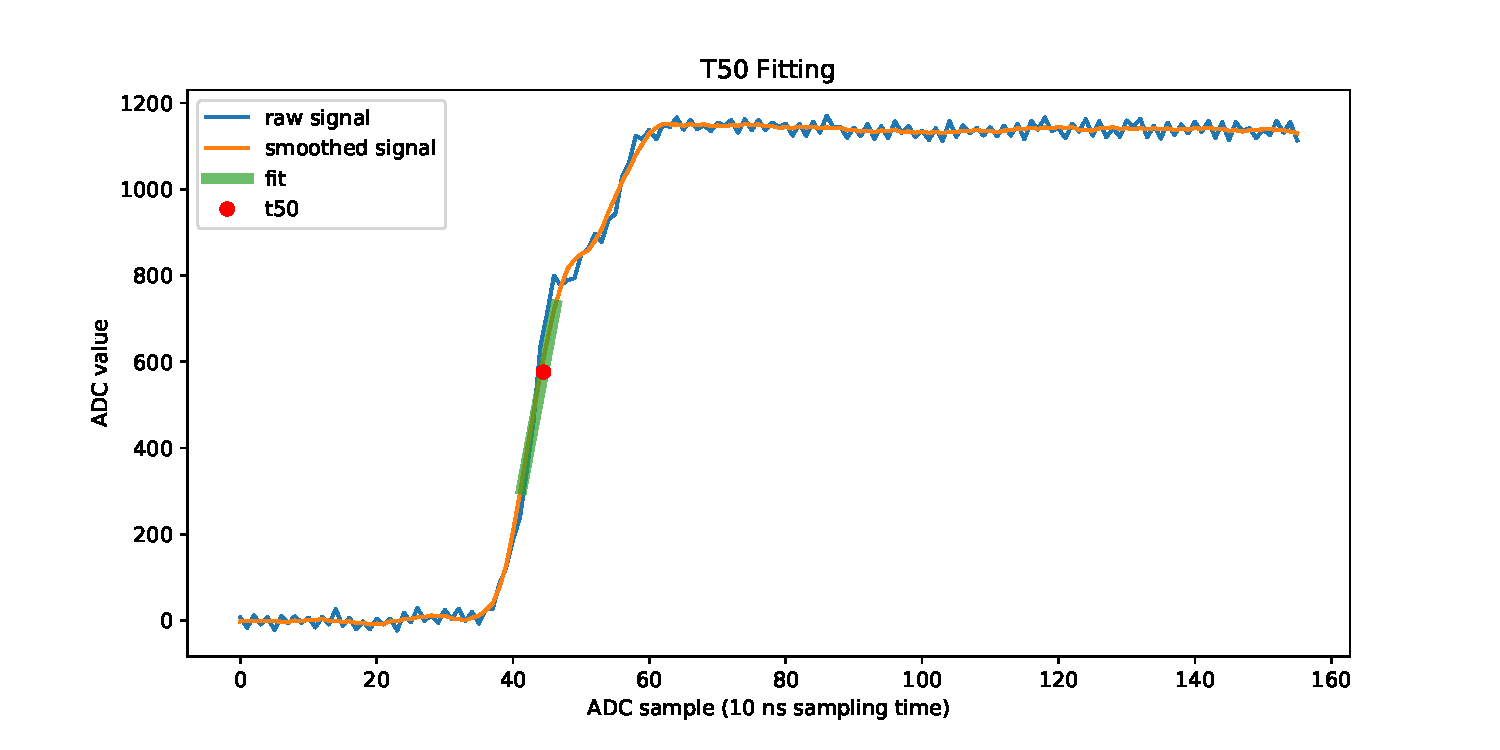
\includegraphics[width=0.7\textwidth]{./figures/t50_fitting.pdf}
\caption{Each raw signal (blue) is smoothed with a Savitzky-Golay filter (orange). The region around the point at which the smoothed signal exceeds half its maximum is fit with a line (green) to extract the t50 value (red point)}
\label{fit}
\end{centering}
\end{figure}


\subsection*{ADL3 Model}

A model of the detector was built using ADL3 (AGATA Demonstrator Library v.3), which uses finite element methods to calculate fields (electric field, electric potential, weighting potential) in the given geometry \cite{adl3}. A 3D model was used, modeling 5 strips on each side. The geometry modeled is show in figure \ref{wpot}, which depicted the weighting potential of the central strip on the DC side. 

This model was used to calculate predicted signals for events taking place at various depths, centered for a strip on either face. A map of the interaction depths simulated is shown in \ref{positions}, where the interaction points are superimposed on the weighting potential plotted in figure \ref{wpot}. Interactions were simulated every 0.1 mm.

The difference in t50 value (time at which the signal reaches half of its maximum) between signals on the central electrode on the AC and DC sides was found for each event. This corresponds roughly to the difference in trigger times expected. In truth, this is an optimistic assumption since effect like the preamplifier response, jitter, charge trapping, etc. are not being taken into account. Using this method, the maximum difference in t50 between the two faces of the crystal is $\approx$ 62 ns. In accordance with this, a coincidence window of 70 ns was used. This slight broadening in time window should not affect the false coincidence rate since a very small fraction of events occur with triggers between 62 and 70 ns ($<$ 0.1 $\%$ ). The expected difference in trigger time is plotted in figure \ref{t50depth}, as a function of interaction depth. The average difference is 31 ns. 

\begin{figure}
\begin{centering}
\includegraphics[width=0.7\textwidth]{./figures/Wpot03.pdf}
\caption{CAPTION}
\label{wpot}
\end{centering}
\end{figure}

\begin{figure}
\begin{centering}
\includegraphics[width=0.7\textwidth]{./figures/positions.pdf}
\caption{CAPTION}
\label{positions}
\end{centering}
\end{figure}

\begin{figure}
\begin{centering}
\includegraphics[width=0.7\textwidth]{./figures/deltat50_vs_depth.pdf}
\caption{CAPTION}
\label{t50depth}
\end{centering}
\end{figure}

\subsection*{Depth Determination}

\subsubsection*{Simple Linear Fit}

The maximum $\Delta t50$was seen to be roughly 210, the minimum $\Delta t50$ was seen to be -160. For a rough determination of the depth, the maximum value is assumed to correspond to the anode and the minimum value to the cathode. A linear fit is applied to determine intermediate position values. This is not a fully representative treatment. It fails to take into account effects due to the non-linear weighting potential directly near electrodes, different charge carrier mobilities, realistic charge transport, and other effects. However, for the purposes of this work, we make this crude assumption following \cite{amman}.

\subsubsection*{Linear Fit}

A different linear interpretation was used as well. Following \cite{cci21}, assuming saturation velocity for both charge carriers, one can use a linear function to relate depth ($z$) to $\Delta t50$:

\begin{equation}
z = z_0 + k \Delta t50
\end{equation}

where z is the depth of the interaction, $z_0$ is a constant depth which is slightly offset from the midpoint of the detector to account for differences in electron and hole velocities, and $k$ is a proportionality factor. $z_0$ and $k$ were experimentally determined for detector 1 to be 5.2 mm and 0.04 mm/ns respectively, in \cite{cci21}. This offset of 5.2 mm was adjusted to 5.95 mm to better fit the data set.

\subsubsection*{Library Method}

Using the ADL3 model and simulated signals described earlier, the depth was calculated using the signal library method. Here, experimental signals were compared to simulated signals to find the simulated signal that most closely matched the measured signal, and assume that interaction depth.

For each event, the signal on a detector face was compared to each simulated signal for that face in the library. The measured signal was shifted in time to most closely match the simulated signal to which is was being compared. This is done because the true start time of the experimental event is not known. In this way, this depth determination method is disentangled from the $\Delta$T50 of an event, and is determine purely from signal shapes.

REDO THIS PLOT TO HAVE LABELS AND TO NOT BE CONCATENATED
\begin{figure}
\begin{centering}
\includegraphics[width=0.7\textwidth]{./figures/simulated_signals.pdf}
\caption{The signals from both faces of the detector are shown here. The positive signals corresponds to the charge induced on the DC electrode, and the negative signals corresponds to that induced on the AC electrode. The blue signals correspond to an event which takes place very near to the DC electrode. The DC signal rises very quickly, and the AC very slowly. The red signal corresponds to an event which takes place very near the AC electrode. Now the AC signal rises very quickly and DC slowly.}
\label{signals}
\end{centering}
\end{figure}

REDO THIS PLOT TO HAVE LABELS 
\begin{figure}
\begin{centering}
\includegraphics[width=0.7\textwidth]{./figures/signal_shift.pdf}
\caption{Here a measured signal (green) has been shifted in time to match a simulated signal (blue). The signal after shifting is shown (red dashed line). It is clear that the measured signal matched better to the library signal after shifting.}
\label{shift}
\end{centering}
\end{figure}
